\subsection{Depth classes of the unsaturated columns}\label{sec:vzclasses}
The soil zone sees the land of a cell at its $N$ DEM samples (Section~\ref{sec:szslope}), but by default each exchange
column has one unsaturated column, starting at the cell's mean soil-zone base. On irregular ground that is a poor
summary: hummocks have a long unsaturated path and hollows a short one; where the mean base lies within $L_{\min}$ of the
water table there is no column at all, and the hummocks' recharge reaches MODFLOW in the step; where the mean base is
far above the water table, the recharge of hollows that are nearly at the water table is delayed as if they were not.
With \cmd{:SoilZoneVadoseClasses} $K$ ($1\le K\le10$, default 1) every exchange column gets up to $K$ unsaturated
columns, one per \emph{depth class} of its DEM samples, for every method (\cmd{RICHARDS}, \cmd{KINEMATIC}, \cmd{LAG}).

\paragraph{Classes.} The samples' soil-zone bases $z_{b,s}$ (ascending) are grouped into at most $K$ contiguous classes
with the least spread: the grouping minimises $\sum_c\sum_{s\in c}(z_{b,s}-\bar z_c)^2$ (Fisher's optimal partition,
found by dynamic programming over the sorted bases). Unlike groups of equal counts it separates real levels, such as
terraces or pits, from the slopes around them. Equal bases are never split, so $K$ is also limited by the number of
distinct bases (with \cmd{:SoilZoneSubgrid 1} or no DEM there is one class). Class $c$ covers the share $a_c=n_c/N$ of
the column; its unsaturated column starts at $z_b+\bar z_c-\bar z$, the class mean shifted with the column's mean base
$z_b$, so the area-weighted mean of the class tops is $z_b$ (the mean depth to the water table is kept) and $K=1$ is the
single column. Its saturated fraction $F_c(h)=\frac1{n_c}\sum_{s\in c}\sigma((h-z_{b,s})/d_s)$ is the column's $F$ (Section~\ref{ch:soilzone}) on the class's own samples, so
$\sum_c a_c F_c=F$ (to round-off; Raven reports the largest deviation in \cmd{GWModelSummary.txt}). The classes are
fixed for the run.

\paragraph{Water.} Class $c$ takes the unsaturated share $a_c(1-F_{0,c})$ of the column's recharge ($F_{0,c}$ at the
start of the step); a class whose column does not exist (its top within $L_{\min}$ of the water table, or below it)
passes its unsaturated share $a_c(1-F_c)$ to the water table in the step and rejects $a_c F_c$, with its fraction at the
connection head (as a column without unsaturated column). Each class column follows the water table as the single
column does (Section~\ref{sec:szvadose}); the limits of the cell that supplies water to a column (its new nodes, a deficit
below a risen water table, upflow) belong to the soil-zone column, so its classes share them: they are processed in
turn and each has what the earlier ones left; the room of the soil-zone layers for capillary rise is shared likewise.
With \cmd{RICHARDS} each class column gives capillary rise from its top node on its unsaturated share; where a class has
no column (and for \cmd{KINEMATIC} and \cmd{LAG} everywhere) the rise comes from the water table to the class's own base.
That rise takes what the source cell's limit (Section~\ref{sec:szvadose}) has left after all the class columns' draws on
it: the water their new nodes took, the negative recharge passed through them and their bottom upflow; one cell never
gives more than that one limit per step (test C11).
The budget columns of the unsaturated zone (inflow, to aquifer, capillary rise, storage) sum all class columns over
their areas $a\,a_c$, and the identities of Chapter~\ref{ch:balance} hold for them as for one column.

\paragraph{Restart.} With $K>1$ the columns are saved in \cmd{solution.rvc} as \cmd{:GWVadoseClassColumns} (HRU ID, cell,
class, classes of the cell, water table, contents; Appendix~\ref{app:hotstart}). A hotstart written with another $K$
(or another node count) does not stop the run: the columns that do not match start at rest (their reference profile)
and Raven warns. A class column that was inactive at the end of the run that wrote the file (the water table fell below
its base in the last step) has no line; the restart builds it at rest, as the continuous run does in its next step, and
this is not a mismatch (\cmd{test\_vz\_classes.py} C10).

\paragraph{Verification} (\texttt{tests/soilzone/test\_vz\_classes.py}; Figure~\ref{fig:vzclasses}). C1: with $K=1$
the outputs are byte-identical to a build without the classes (\cmd{NONE}, and \cmd{RICHARDS} where the water table does
not reach, within a step, ground unsaturated at its start; elsewhere the hand-back of rule (i), Section~\ref{sec:szvadose},
is the only difference), the diagnostic column \emph{interface change} left out. C2: a cell with hummocks of $\pm2.5$~m
whose mean base is 3~cm above the water table: with $K=1$ no water passes through a column; with $K=3$ 949~m$^3$ pass
through the hummocks' columns, their outflow 1.79~d after their inflow, with $K=5$ 5\,558~m$^3$ (0.35~d: more of the
area is in short columns). C3: the recharge to MODFLOW approaches the one with every sub-area modelled by its own column
as $K$ grows: nine random squares per cell ($\pm1$~m, water table 1.3~m deep) against $K=9$ (one class per square; with
$5\times5$ samples one class per square would need $K=25$, beyond the limit of 10): relative error 0.0025, 0.00066,
0.00037, 3.6\,$\times10^{-5}$, 3.3\,$\times10^{-5}$, 2.0\,$\times10^{-5}$ and 1.1\,$\times10^{-6}$ for $K=1,2,3,4,5,6,8$;
two terraces 1.2~m apart: 0.0029 with $K=1$ ($K=2$ exact); squares of $\pm1.4$~m over a water table 3~m deep: 0.14,
0.013, 0.0025 and 0.0004 for $K=1,2,4,6$. C4: capillary rise from four class columns under evaporation; C5: water tables
rising and falling through the class columns of four HRUs (shared limits); C6: a specified-head toe, a dried thin top
layer (\cmd{SZW\_RAVEN}), a restart with $K=3$ (20 + 20 days against 40: largest deviation $1.7\times10^{-8}$) and hotstarts
written with $K=1$ read with $K=3$ and vice versa (warning, no stop); C8: \cmd{KINEMATIC} and \cmd{LAG} with $K=3$. In all
of them MODFLOW's balance closes and the recharge, soil-zone and column identities stay below $10^{-8}$ (C4 and C8 below
$10^{-9}$). C7: the cost grows less than in proportion to $K$ (small test cases: 0.32, 0.49 and 0.48~s for $K=1,3,5$;
timings depend on the machine and its load). C9 runs the rough-terrain regression case R20 (\cmd{band\_e43}, an existing
model whose sub-grid bases lie just above the top cell's bottom, \cmd{LAG}) with three classes through
\cmd{test\_rough\_terrain.py}: it checks the interface's connection head (Section~\ref{ch:soilzone}); the saturated
fraction follows the independent closure on converged steps within R20's limit 0.004 (0.0001; a connection head left above
MODFLOW's head gave 0.51).

\begin{figure}[!htbp]\centering
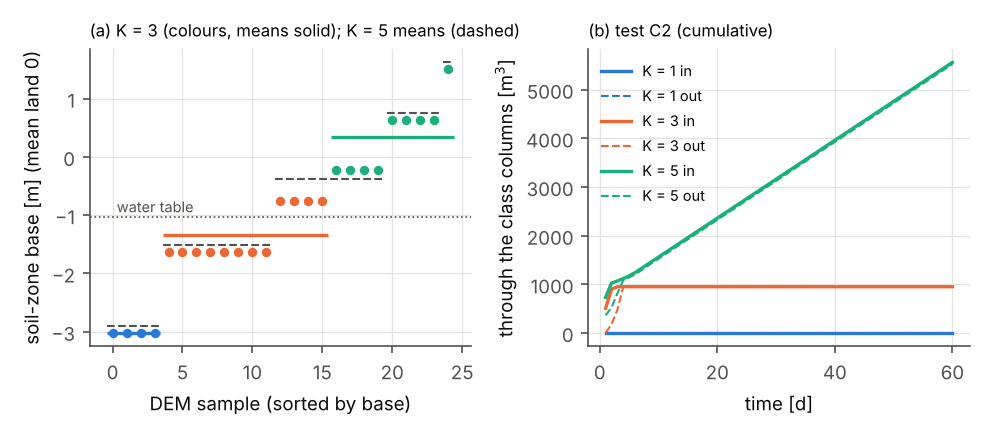
\includegraphics[width=\linewidth]{figures/fig_vz_classes.png}
\caption{Depth classes. (a) The 25 samples of a hummocky cell (test C2), sorted by their soil-zone base, grouped with the least spread
into 3 classes (colours; solid lines: class means) and into 5 (dashed lines: class means, drawn slightly above). (b) Test C2: water entering (solid) and leaving (dashed) the class columns,
cumulative; with $K=1$ the cell has no column.}\label{fig:vzclasses}
\end{figure}

\paragraph{Reference card.} \cmd{:SoilZoneVadoseClasses} $K$ ($1\le K\le10$; default 1: one column per exchange column
at its mean base); classes by least spread of the DEM samples' bases; class $c$: area $a_c$, top at its mean base,
inflow $a_c(1-F_c)$; a class without column passes its share to the water table; limits of the source cell and room of
the soil layers shared by the classes; hotstart \cmd{:GWVadoseClassColumns}.
